\documentclass{if-beamer}

% --------------------------------------------------- %
%                  Presentation info	              %
% --------------------------------------------------- %
\title[Lecture 19]{Lecture 19}
\subtitle{Integration: Simpson's 1/3 Rule, Simpson's 3/8 Rule}
\author{Ashley Gannon}
\date{ISC3313 Fall 2021}
\logo{

\includegraphics[scale=0.08]{figures/FSULogo.png}
}
\subject{Presentation subject}

% --------------------------------------------------- %
%                    Title + Schedule                 %
% --------------------------------------------------- %
\begin{document}

\begin{frame}
  \titlepage
\end{frame}
% --------------------------------------------------- %
%                      Presentation                   %
% --------------------------------------------------- %
\section{The Composite Simpson's 1/3 Rule Continued}

\begin{frame}
\frametitle{Let's think back to our formula}
The total integration using Simpson's 1/3 Rule can be represented as
$$I = \frac{h}{3}(f(x_0)+f(x_n))+\frac{h}{3}\left( 4\sum_{i = 1,3,5...}^{n-1}f(x_i) + 2\sum_{j = 2,4,6,...}^{n-2} f(x_j) \right)$$
with error
$$ E_a = -\frac{(b-a)^5}{180n^4}\bar{f}^{(4)}$$.
\end{frame}

\begin{frame}
	\frametitle{Let's think back to our formula}
	The total integration using the composite Simpson's 1/3 Rule can be represented as
	$$I = \frac{h}{3}(f(x_0)+f(x_n))+\frac{h}{3}\left( 4\sum_{i = 1,3,5...}^{n-1}f(x_i) + 2\sum_{j = 2,4,6,...}^{n-2} f(x_j) \right)$$
	with error
	$$ E_a = -\frac{(b-a)^5}{180n^4}\bar{f}^{(4)}$$
	Thinking back to the total integration using the composite trapezoid rule
	$$ I = \frac{h}{2}*(f(x_0)+f(x_n))+h\sum_{i=1}^{n-1}f(x_i)$$ 
	with error
	$$E_a = -\frac{(b-a)^3}{12n^2}\bar{f}''$$
\end{frame}

\begin{frame}
	\frametitle{Let's think back to our formula}
	The total integration using the composite Simpson's 1/3 Rule can be represented as
	$$I = \frac{h}{3}(f(x_0)+f(x_n))+\frac{h}{3}\left( 4\sum_{i = 1,3,5...}^{n-1}f(x_i) + 2\sum_{j = 2,4,6,...}^{n-2} f(x_j) \right)$$
	with error
	$$ E_a = -\frac{(b-a)^5}{180n^4}\bar{f}^{(4)}$$
	Thinking back to the total integration using the composite trapezoid rule
	$$ I = \frac{h}{2}*(f(x_0)+f(x_n))+h\sum_{i=1}^{n-1}f(x_i)$$ 
	with error
	$$E_a = -\frac{(b-a)^3}{12n^2}\bar{f}''$$
	We notice that the only big difference between these methods is that the odd \textbf{index values} of $x_i$ carry a different coefficient for the $f(x_i)$ values than they do when they are even. So we need to add this conditional to our for loop. 
\end{frame}

\begin{frame}
	\frametitle{I bolded \textbf{index values} in the last slide because}
	\begin{figure}
		\centering
		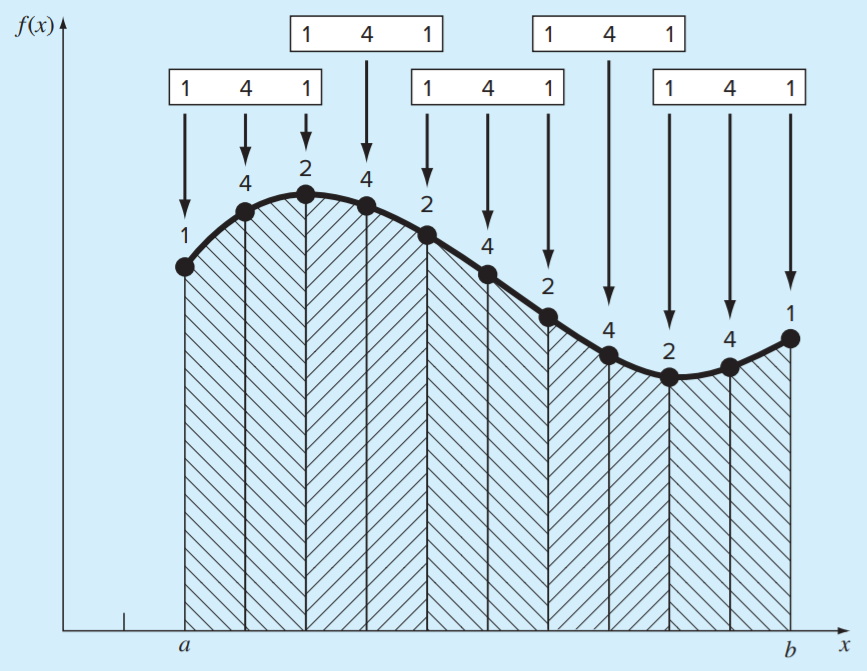
\includegraphics[width = .8\textwidth]{figures/compsimp}
	\end{figure}
\end{frame}

\begin{frame}
	\frametitle{The Modulo Operator, \%}
	\begin{itemize}
		\item One way to tell if a number is even is to use the modulo operator \%. \\\vspace{10pt}
		\item The modulo operator gives the remainder of a division between two values. \\\vspace{10pt}
		\begin{itemize}
			\item \texttt{x = 31 \% 4} would result in \texttt{x} being equal to \texttt{3} since 31/4 = 7R3. \\\vspace{10pt}  
		\end{itemize}
		\item Now, if a number \texttt{n} is even, we expect that in the case of \texttt{x = n \% 2}, \texttt{x} would be equal to \texttt{0}. \\\vspace{10pt}
		\item Knowing this information now, we can use this to form a conditional statement that evaluates whether a number is even \\\vspace{10pt}
		\begin{itemize}
			\item \texttt{if (x \% 2 == 0)}
		\end{itemize}
	\end{itemize}
\end{frame}

\begin{frame}
	\frametitle{Recursive Simpson's 1/3 Rule Pseudocode}
	\texttt{declare function that takes in a, b, n, $\bar{f}^{(4)}$, tolerance}\\
	\texttt{ }
	\\\texttt{declare/define the error $-\frac{(b-a)^5}{180n^4}* \bar{f}^{(4)}$}\\\vspace{2pt}
	\texttt{if error > tolerance}\\
	\texttt{This is where recursion comes in}\\
	\texttt{\qquad redefine n, n = 2*n for example}\\
	\texttt{\qquad return function(a,b,n,$\bar{f}^{(4)}$, tol)}\\
	\texttt{ } \\
	\texttt{declare/define h = (b-a)/n;}\\
	\texttt{declare/define sum = (h/3)*(f(a)+f(b)); }\\
	\texttt{declare/define xi = a+h;}\\
	\texttt{ }\\
	\texttt{loop over i = 1,...,n-1 }\\
	\texttt{\qquad if(i \% 2 == 0)}\\
	\texttt{\qquad \qquad add 2*h/3*f(xi) to sum} \\
	\texttt{\qquad else}\\
	\texttt{\qquad \qquad add 4*h/3*f(xi) to sum} \\
	\texttt{\qquad update xi = xi +h;}\\
\end{frame}

\begin{frame}
	\frametitle{Applying it to our problem}
	Let's apply our code to our problem from last class:
	$$f(x) =0.2+25x-200x^2+675x^3-900x^4+400x^5$$
	from $a = 0$ to $b=0.8$, with $\bar{f}^{(4)} = -24000$, $n=2$ and $tol = 0.00001$.
\end{frame}

\begin{frame}
	\frametitle{Applying it to our problem}
	Let's apply our code to our problem from last class:
	$$f(x) =0.2+25x-200x^2+675x^3-900x^4+400x^5$$
	from $a = 0$ to $b=0.8$, with $\bar{f}^{(4)} = -24000$, $n=2$ and $tol = 0.00001$.\\\vspace{1cm}
	
	We notice this method required a 16 times less segments to reach the specified tolerance.
	\begin{itemize}
		\item Composite Trapezoid: 512
		\item Composite Simpson's 1/3: 32
	\end{itemize}
	
\end{frame}

\begin{frame}
	\frametitle{}
	\begin{itemize}
		\item The composite version of Simpson’s 1/3 rule is considered superior to the trapezoidal rule for most applications.\\\vspace{10pt}
		\item As mentioned previously, it is
		limited to cases where the values are equispaced. \\\vspace{10pt}
		\item Further, it is limited to situations where
		there are an even number of segments and an odd number of points. \\\vspace{10pt}
		\item  Consequently, an odd-segment–even-point formula known as Simpson’s 3/8 rule can be used in conjunction with the 1/3 rule to permit evaluation of both even and odd numbers of equispaced segments.
	\end{itemize}
\end{frame}

\section{Simpson's 3/8 Rule}
\begin{frame}[t]
	\frametitle{Simpson's 3/8 Rule}
	In a similar manner to the derivation of the trapezoidal and Simpson’s 1/3 rule, a third-order Lagrange polynomial can be fit to four points and integrated to yield
	$$I =\frac{3h}{8}[f(x_0)+3f(x_1)+3f(x_2)+f(x_3)]$$
	where $h=(b-a)/3$. This equation is known as Simpson's 3/8 rule because h is multiplied
	by 3/8. It is the third Newton-Cotes closed integration formula. \\\vspace{10pt}
	
	Simpson’s 3/8 rule has an error of
	$$E_a = -\frac{(b-a)^5}{6480}\bar{f}^{(4)} $$ 
	Because the denominator is larger than for Simpson's 1/3 Rule, 
	$$E_a = -\frac{(b-a)^5}{2880}\bar{f}^{(4)} $$
	the 3/8 rule is somewhat more accurate than the 1/3 Rule.
\end{frame}

\begin{frame}
	\frametitle{When do we use it?}
	We've written the Trapezoid Rule and Simpson's 1/3 Rule to integrate functions, where we are able to use recursion to find the value of n that reduces our error below our tolerance.\\\vspace{10pt}
	
	What if now our problem is to integrate over an even set of data values where the number of segments is not divisible by three?
	\begin{itemize}
		\item We would have an odd number of segments, so we wouldn't be able to only use Simpson's 1/3 method alone since segments aren't divisible by 2 
		\item and we wouldn't be able to use Simpson's 3/8 method alone since the number of segments isn't divisible by 3.
		\item We can evaluate this data set using a combination of Simpson's 1/3 Rule and Simpson's 3/8 Rule. 
	\end{itemize}   
\end{frame}

\begin{frame}
	\frametitle{Example Problem}
	Let's say we've got a set of data we want to integrate
	\begin{table}
		\begin{tabular}{c| c c c c c c c c}
		$i$ &0& 1&2&3&4&5&6&7 \\
		\hline
		$x_i$& 1.0 &1.1&1.2&1.3&1.4&1.5&1.6&1.7\\
		$f(x_i)$&1.543&1.669&1.811&1.971&2.151&2.352&2.577&2.828\\

		\end{tabular}
	\end{table}
\end{frame}

\begin{frame}
	\frametitle{Example Problem}
	Let's say we've got a set of data we want to integrate
	\begin{table}
		\begin{tabular}{c| c c c c c c c c}
			$i$ &0& 1&2&3&4&5&6&7 \\
			\hline
			$x_i$& 1.0 &1.1&1.2&1.3&1.4&1.5&1.6&1.7\\
			$f(x_i)$&1.543&1.669&1.811&1.971&2.151&2.352&2.577&2.828\\
			
		\end{tabular}
	\end{table}
The first thing we need to do is divide the interval between the two methods. \\\vspace{5pt}
\begin{itemize}
	\item We'll reserve the last 3 segments for Simpson's 3/8 Rule.
	\item The remaining 4 segments (the first four segments) will be evaluated using Simpson's 1/3 Rule.
	\item This method is still 4th order accurate.
\end{itemize}
\end{frame}

\begin{frame}
	\frametitle{Example Problem}
	Let's say we've got a set of data we want to integrate
	\begin{table}
		\begin{tabular}{c| c c c c c c c c}
			$i$ &0& 1&2&3&4&5&6&7 \\
			\hline
			$x_i$& 1.0 &1.1&1.2&1.3&1.4&1.5&1.6&1.7\\
			$f(x_i)$&1.543&1.669&1.811&1.971&2.151&2.352&2.577&2.828\\
			
		\end{tabular}
	\end{table}
	The first thing we need to do is divide the interval between the two methods. \\\vspace{5pt}
 	\begin{enumerate}
 		\item Use Simpson's 1/3 rule on the interval [1.0,1.4]. From our data, $h = 1.1-1.0 = 0.1$.
 		\begin{align*}
 		\int_{1.0}^{1.4}f(x)dx &\approx\frac{h}{3}\bigg(f(x_0)+4f(x_1)+2f(x_2)+4f(x_3)+f(x_4)\bigg)\\
 		&=\frac{0.1}{3}\bigg(1.543+4(1.669)+2(1.811)+4(1.971)+2.151\bigg)\\
 		&=0.729200\\
 		\end{align*}
 	\end{enumerate}	
\end{frame}

\begin{frame}
	\frametitle{Example Problem}
	Let's say we've got a set of data we want to integrate
	\begin{table}
		\begin{tabular}{c| c c c c c c c c}
			$i$ &0& 1&2&3&4&5&6&7 \\
			\hline
			$x_i$& 1.0 &1.1&1.2&1.3&1.4&1.5&1.6&1.7\\
			$f(x_i)$&1.543&1.669&1.811&1.971&2.151&2.352&2.577&2.828\\
			
		\end{tabular}
	\end{table}
	The first thing we need to do is divide the interval between the two methods. \\\vspace{5pt}
	\begin{enumerate}[2]
		\item Use Simpson's 3/8 rule on the interval [1.4,1.7]. From our data, $h = 1.1-1.0 = 0.1$.
		\begin{align*}
		\int_{1.4}^{1.7}f(x)dx &\approx\frac{3h}{8}\bigg(f(x_4)+3f(x_5)+3f(x_6)+f(x_7)\bigg)\\
		&=\frac{3(0.1)}{3}\bigg(2.151+3(2.352)+3(2.577)+2.828\bigg)\\
		&=0.741225\\
		\end{align*}
	\end{enumerate}	
\end{frame}

\begin{frame}
	\frametitle{Example Problem}
	Let's say we've got a set of data we want to integrate
	\begin{table}
		\begin{tabular}{c| c c c c c c c c}
			$i$ &0& 1&2&3&4&5&6&7 \\
			\hline
			$x_i$& 1.0 &1.1&1.2&1.3&1.4&1.5&1.6&1.7\\
			$f(x_i)$&1.543&1.669&1.811&1.971&2.151&2.352&2.577&2.828\\
			
		\end{tabular}
	\end{table}
	The first thing we need to do is divide the interval between the two methods. \\\vspace{5pt}
	\begin{enumerate}[3]
		\item Add them together.
		\begin{align*}
		\int_{1.0}^{1.7}f(x)dx &\approx \int_{1.0}^{1.4}f(x)dx + \int_{1.4}^{1.7}f(x)dx\\
		&=1.47042\\
		\end{align*}
	\end{enumerate}	
\end{frame}


\begin{frame}
	\frametitle{Example Problem}
	Let's say we've got a set of data we want to integrate
	\begin{table}
		\begin{tabular}{c| c c c c c c c c}
			$i$ &0& 1&2&3&4&5&6&7 \\
			\hline
			$x_i$& 1.0 &1.1&1.2&1.3&1.4&1.5&1.6&1.7\\
			$f(x_i)$&1.543&1.669&1.811&1.971&2.151&2.352&2.577&2.828\\
			
		\end{tabular}
	\end{table}
	The first thing we need to do is divide the interval between the two methods. \\\vspace{5pt}
	\begin{enumerate}[3]
		\item Add them together.
		\begin{align*}
		\int_{1.0}^{1.7}f(x)dx &\approx \int_{1.0}^{1.4}f(x)dx + \int_{1.4}^{1.7}f(x)dx\\
		&=1.47042\\
		\end{align*}
	\end{enumerate}	
Alternatively, we could have used Simpson’s 3/8 rule on the fist three segments, [1.0, 1.3], and Simpson’s 1/3 rule on the remaining 4 segments, [1.3, 1.7]. We would obtain a slightly different approximation: 1.4704416. Either way works, they are both accurate up to the 4th decimal. 
\end{frame}

\begin{frame}
	\frametitle{Things to consider before we code}
	We want to write a \texttt{DataSimpsonSRules} function that will evaluate both odd and even sets of data. 
		\begin{itemize}
			\item Our function will have to take in arrays for $x$ and $f(x)$ values.
			\item We will have to use the number of x values in these arrays to figure out how many segments,$n$, our domain has. 
			\item We will need to set up different cases for when $n$ is even, odd and divisible by 3, or odd and not divisible by 3 and evaluate the sum for the appropriate case. \\\vspace{10pt}
		\end{itemize}
	Think about how you might approach this between now and next class.
\end{frame}

\end{document}
